\section{Studio della mappa logistica}%
La mappa logistica è definita come
\[
x_{n+1} = 4\alpha x_n(1-x_n) = G(x_n) \qquad  \alpha  \in \left] 0, 1\right], \quad  x \in \left[0, 1\right]
.\] 
Spesso useremo la notazione equivalente con $\mu =4\alpha$.\\
Essendo una mappa quadratica sappiamo che non è invertibile, vedremo che è proprio questa caratteristica a renderla interessante.\\
Troviamone gli stati stazionari:
\[
    x = 4\alpha x(1-x) \implies  x\left[1-4\alpha + 4\alpha x\right] = 0
.\] 
Quindi si ha:
\[\begin{aligned}
    &x_{s_1}=0  && \forall \alpha \\
    &x_{s_2} = \frac{4\alpha-1}{4\alpha} = 1 - \frac{1}{4\alpha} && \text{ Se } 4\alpha-1 > 0
.\end{aligned}\]
Valutiamo la stabilità di questi due stati:
\[
    \left. \frac{\text{d} G}{\text{d} x} \right|_{x = x_{s}} = 4\alpha  - 8 \alpha  x_s
.\] 
Per i nostri stati in particolare:
\[
    \left. \frac{\text{d} G}{\text{d} x} \right|_{x=x_{s_1}} = 4\alpha  \implies  0 < 4\alpha  < 1 \quad
	\begin{dcases}
	\text{ Stabile} \implies  \alpha  < \frac{1}{4}\\
	\text{ Instabile} \implies  \alpha  > \frac{1}{4}\\
	\end{dcases}
.\] 
Quindi notiamo subito che per $\alpha  = 1 /4$ c'è un cambio di stabilità per questo stato stazioario, questo fenomeno è proprio quello che da origine alla famosa \textbf{biforcazione}. Prendiamo l'altro stato stazioario:
\[
    \left. \frac{\text{d} G}{\text{d} x} \right|_{x=x_{s_2}} = 2-4\alpha  \implies  2 \left|1-2\alpha\right| < 1 
	\quad 
	\begin{dcases}
	\text{ Stabile} \implies  \frac{1}{4}< \alpha  < \frac{3}{4}\\
	\text{ Instabile} \implies  \text{ fuori..}
	\end{dcases}
.\] 
Determiniamo adesso se esistono orbite di periodo 2 della mappa logistica. Dobbiamo costruire una $Q(x)$ tale per cui:
\[
    Q(x)  = G^2(x) = G(G(x)) 
.\] 
Le orbite di periodo $2$ se esistono sono definite da $x = Q(x)$. \\
\subsection{Stati instabili della mappa logistica ed introduzione alle biforcazioni.}%
Riscriviamo la mappa con la notazione:
\[
    x_{n+1} = \mu x_n(1-x_n) \quad  \mu  \in \left]0, 4\right] \quad  x \in \left[0, 1\right]
.\] 
E prendiamo lo stato instabile:
\[
    x_{s_2} = \frac{\mu-1}{\mu} \quad  \mu  > 3
.\] 
In questo caso non esiste nessuno stato stazioario stabile, in questo caso la mappa potrebbe presentare il caos oppure potrebbe oscillare tra stati stazionari\ldots\\
Indaghiamo quindi quello che avviene alla mappa nel caso di $\mu >3$ utilizzando due metodi numerici:
\begin{description}
    \item [Metodo CopWeb]: Metodo grafico per comprendere il comportamento della mappa.	
\marginpar{
        \captionsetup{type=figure}
        \fbox{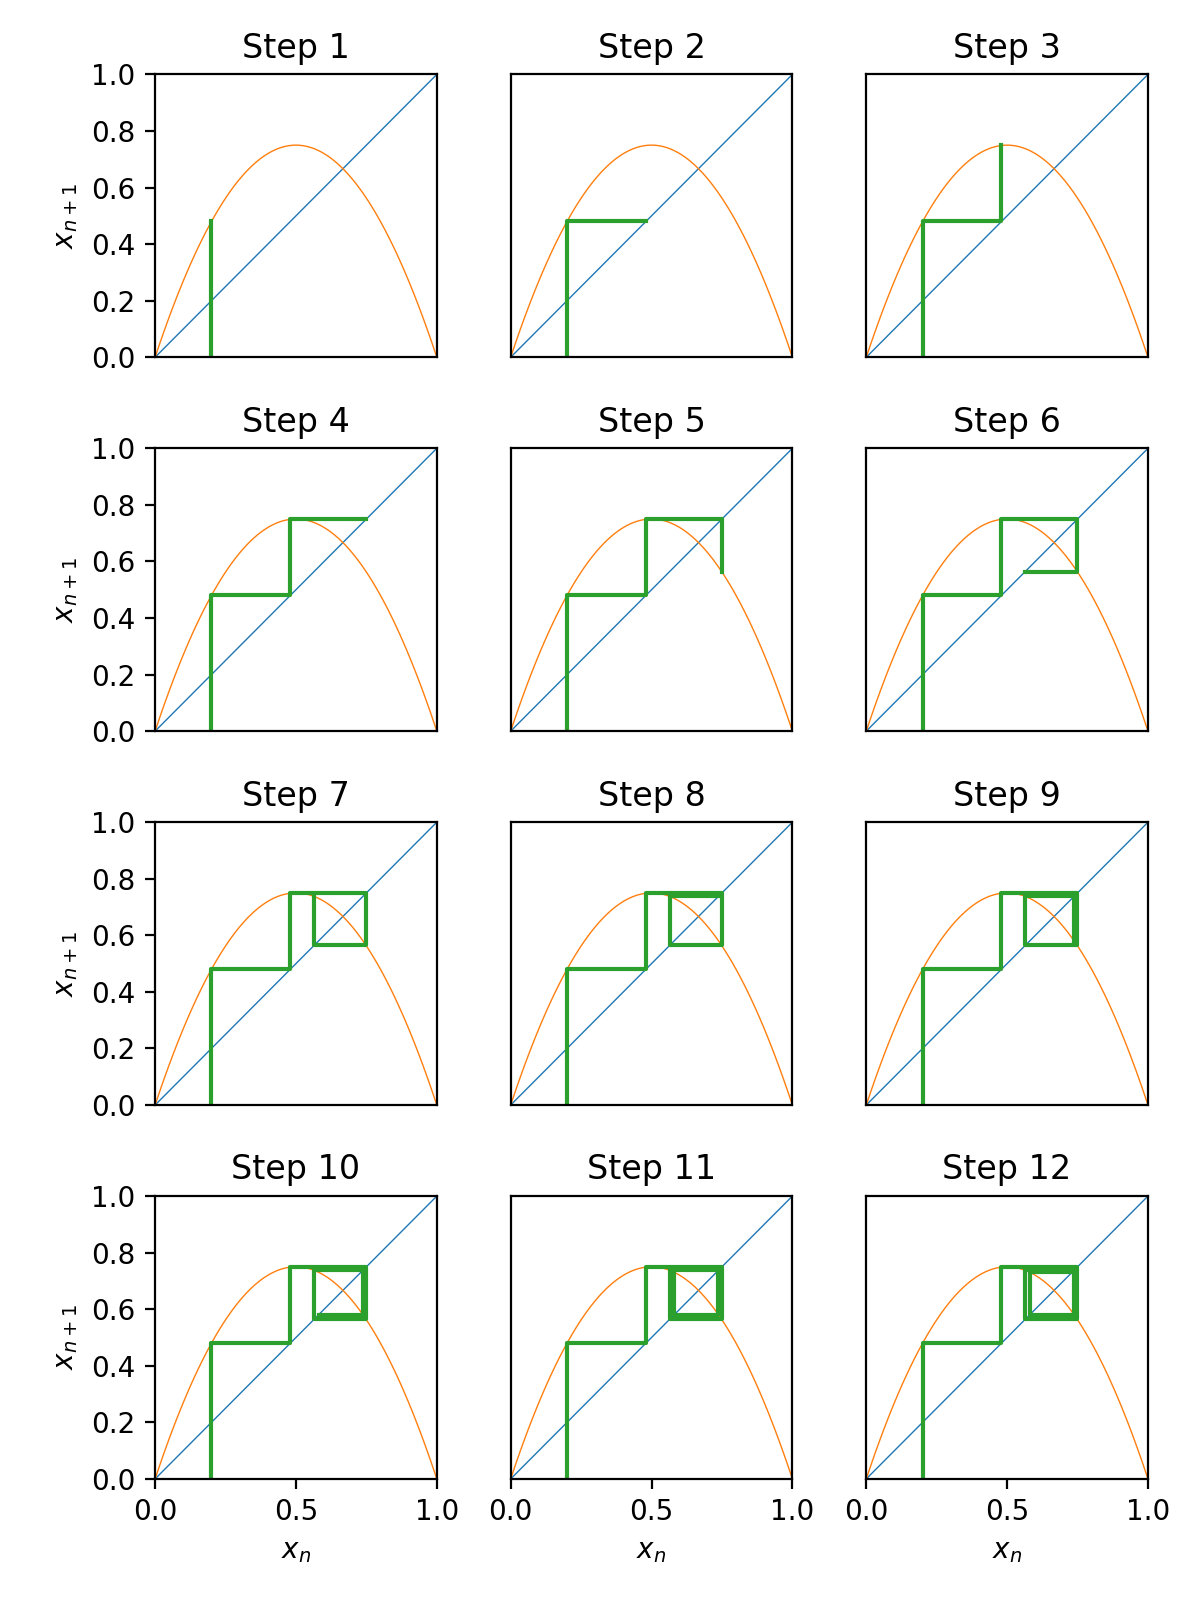
\includegraphics[width=\marginparwidth]{figures/chap3/3_3_1.png}}
        \caption{\scriptsize Esempio di Metodo Cobweb per la mappa logistica con $\mu > 3$}
    \label{fig:3_3_1}
}
    \item [Diagramma di Biforcazione]: un diagramma che ci consense di capire i possibili comportamenti della mappa al variare di $\mu$ (simulandola).
\end{description}
Partiamo dal primo dei due, per sfruttare questo metodo si traccia prima la costruzione geometrica di figura \ref{fig:3_3_4}. L'intersezione tra la parabola (che rappresenta la mappa) e la retta $y=x$ sono i punti fissi della mappa.\\
Se $\mu < 1$ tale disegno non vale, questo perché lo stato stazionario $x_{s_2}$ (quello in alto) smette di esistere e rimane solo quello nell'origine.\\
Graficamente questo fatto può essere attribuito alla derivata della parabola che, per $\mu < 1$ non permette alla parabola di intersecare la retta in punti diversi dall'origine.
\marginpar{
        \captionsetup{type=figure}
        \incfig{3_3_4}
        \caption{\scriptsize Dettagli di costruzione del metodo Cobweb con $\mu >1$.}
    \label{fig:3_3_4}
    }
La mappa evolve geometricamente come in Figura \ref{fig:3_3_1}: si tratta di proiettare iterativamente sulla parabola e sulla retta in maniera alterna con rette verticali e orizzontali. In particolare il caso in tale figura è tale per cui il punto stazionario $x_{s_2}$ non è più stabile, si ha una oscillazione attorno a tale stato.\\
\begin{figure}[H]
    \centering
    \fbox{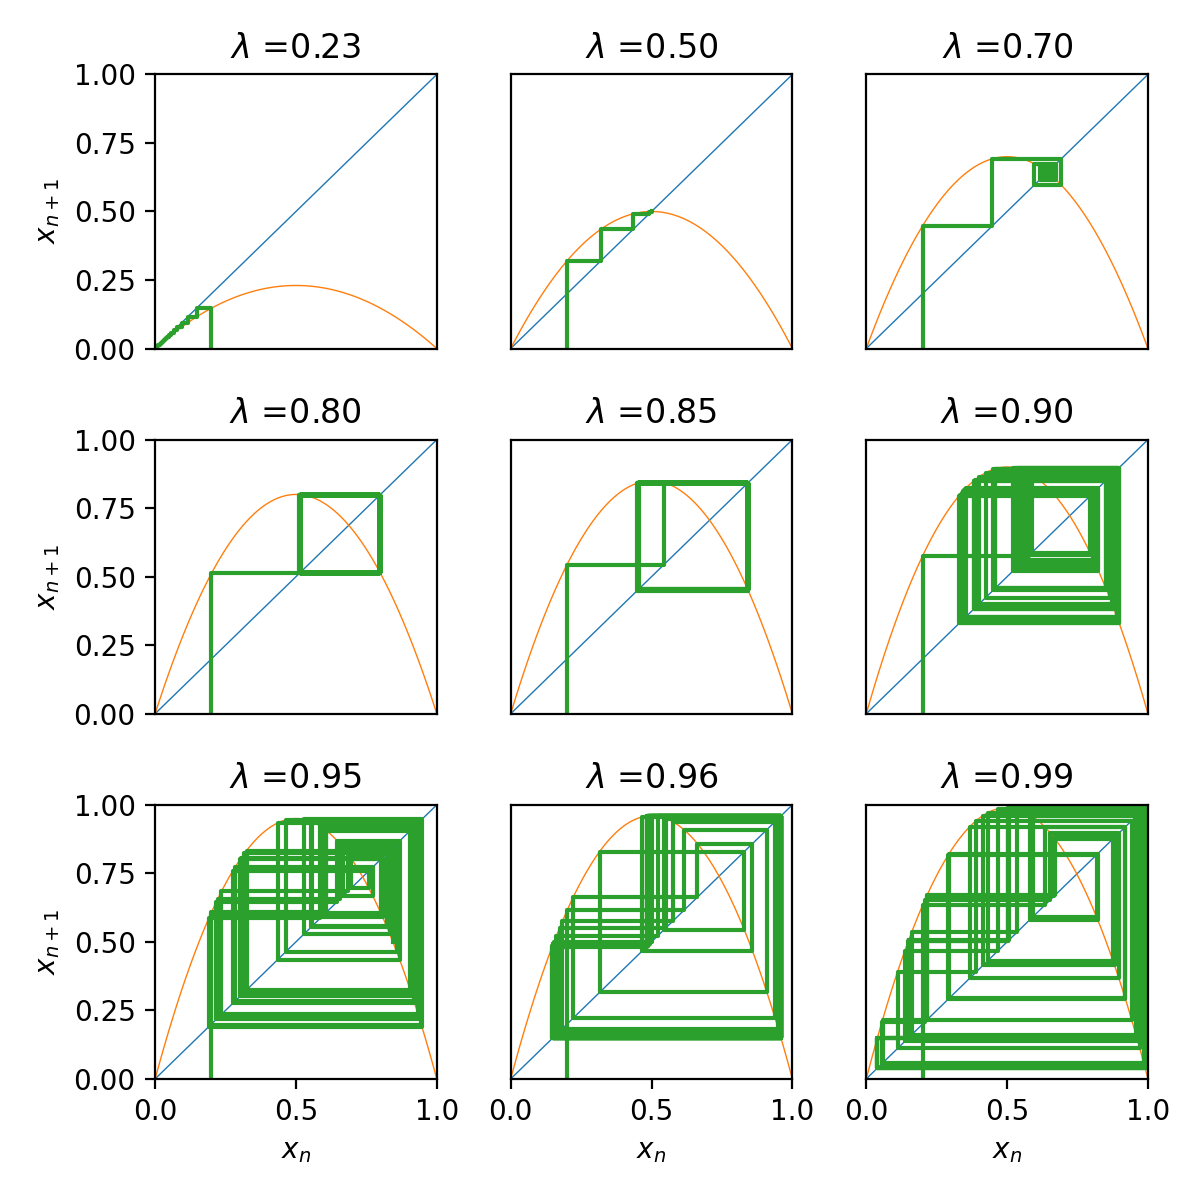
\includegraphics[width=\textwidth]{figures/chap3/3_3_2.png}}
    \caption{\scriptsize Rappresentazione della Cobweb per vari valori di $\lambda  = \mu  / 4$. Notare la ricchezza di comportamenti che può assumere questa semplice mappa.}
    \label{fig:3_3_3}
\end{figure}
\noindent
Il secondo approccio (grafico di Biforcazione) consiste nel fare, di forza bruta, il calcolo numerico di tutti i punti della mappa.
\begin{enumerate}
    \item Si sceglie un numero di intervalli $N_I$ in cui suddividere l'intervallo $\left]0, 4\right]$\sidenote{\scriptsize Maggiore è $N_I$ e più sarà nitida la rappresentazione.}.
\item $\forall \mu_i \in \left]0, 4\right]$ si itera la mappa $N_T$ volte con $N_T$ "sufficientemente grande" ed i valori ottenuti non vengono presi in considerazione (valori transienti)\sidenote{\scriptsize Per vedere se $N_T$ è sufficiente si procede raddoppiandolo o dimezzandolo: se i risultati cambiano con queste due operazioni allora non ci siamo ancora\ldots}
\item Si eseguono altre $N_B$ iterazioni e per ognuna di queste si memorizza lo stato.
\end{enumerate}
In questo modo si associa ad ogni $\mu$ un vettore del tipo:
\[
    \forall \mu  \in \left]0, 4\right] \to \v{S} = \begin{pmatrix} x_{N_T + 1} \\ x_{N_T + 2} \\ \vdots \\ x_{N_T + N_B} \end{pmatrix}
.\] 
In fine tali valori memorizzati vengono inseriti in un grafico $x_n$ vs $\mu_i$ $\forall \mu_i \in \left]0, 4\right]$  (con il passo di $N_I$).\\
Il risultato è mostrato in figura \ref{fig:3_3_3}:
\begin{figure}[H]
    \centering
    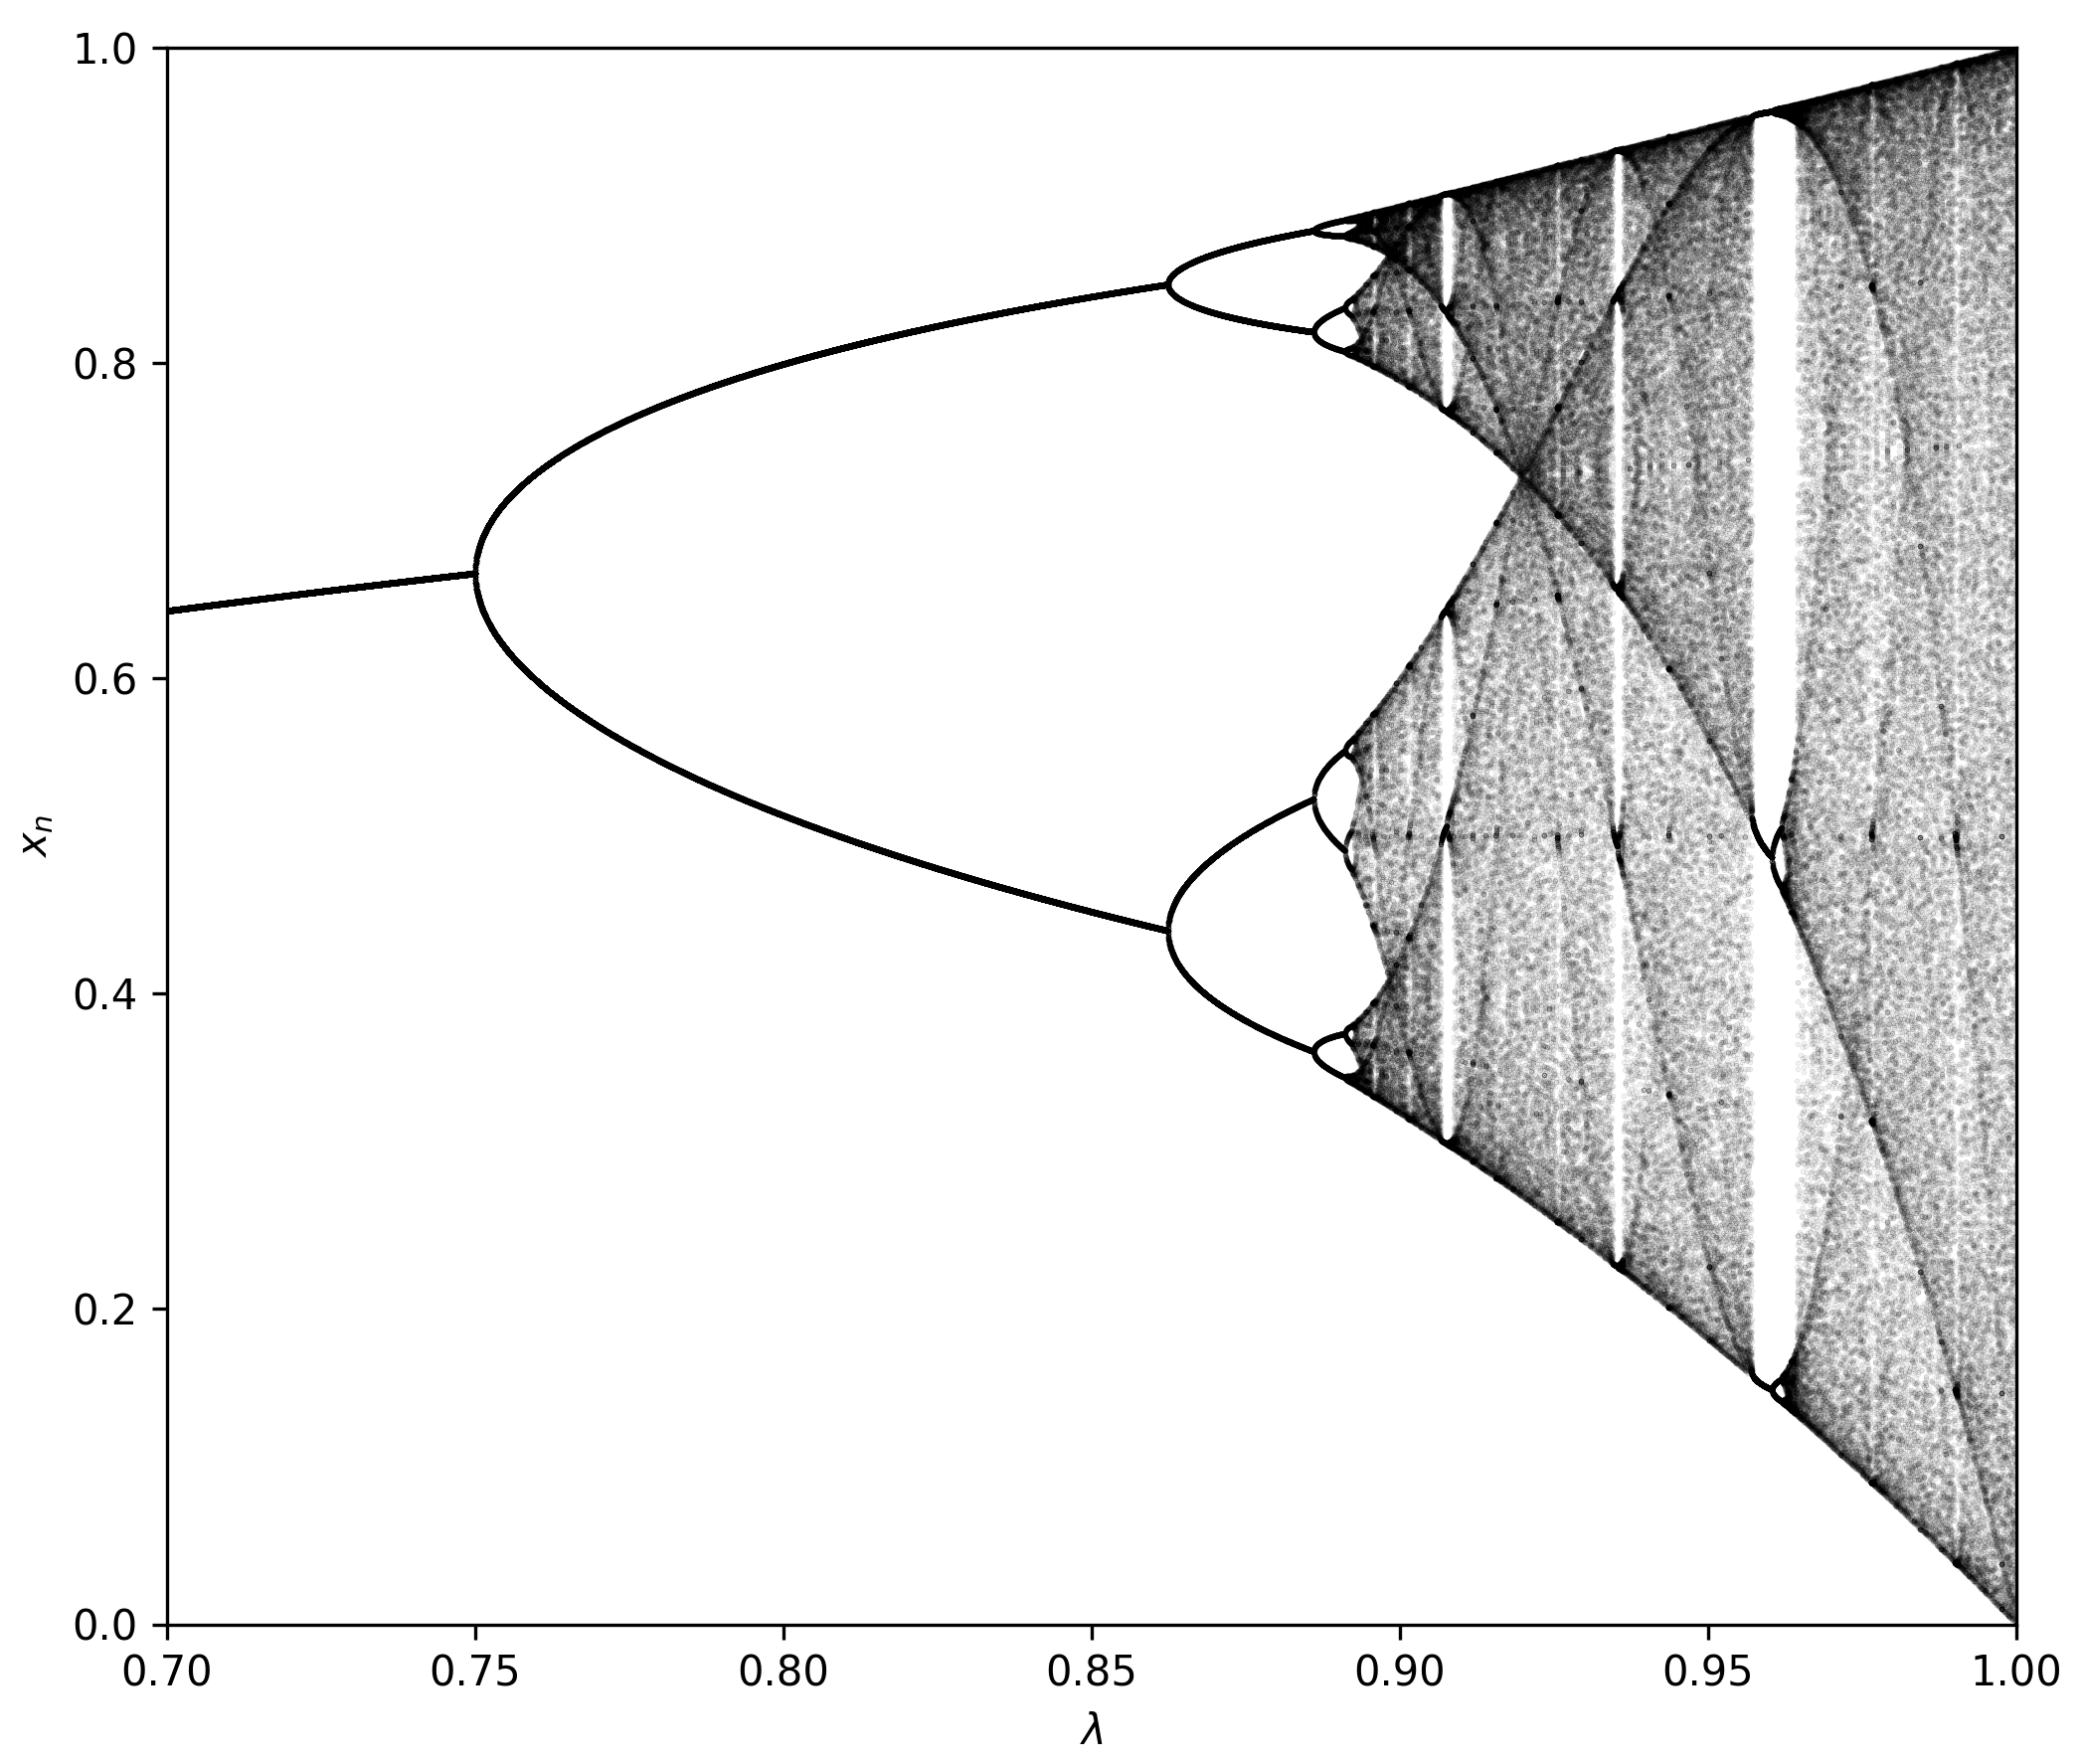
\includegraphics[width=\textwidth]{figures/chap3/3_3_3.png}
    \caption{\scriptsize Grafico di Biforcazione per la mappa Logistica.}
    \label{fig:3_3_3}
\end{figure}
\noindent
In figura osserviamo che, ponendoci ad esempio a $\alpha  \equiv \lambda  = 0.87$ (quindi a $\mu\simeq 3.48$) il sistema oscilla tra 4 punti: fa una orbita 4 periodica!\\
Aumentando $\mu$ anche questa orbita 4 periodica va incontro a instabilità: ogni ramo si biforca nuovamente fino ad uno stato 8 periodico. Si ha quindi una esplosione esponenziale del periodo dell'orbita all'aumentare di $\mu$.\\
Intorno a $\mu\simeq 3.55$ l'orbita diventa essenzialmente $\infty$ periodica: caos deterministico.\\
Dimostriamo che, se consideriamo l'orbita di periodo 2, si ottengono gli stati stazionari presenti in figura per $0.75\lesssim \alpha\lesssim 0.87$. Per farlo definiamo nuovamente 
\[
    Q(x) = G(G(x)) = G^2(x) \implies  x_{n+1} = Q(x_n) 
.\] 
Per definizionde di $Q$ si ha che se $x_1 = \mu x(1-x)$ allora:
\[
    Q(x) = \mu x_1(1-x_1) = \mu\left[\mu x(1-x)\right](1-\left[\mu x(1-x) \right]) 
.\] 
Sviluppando i conti si cconclude che:
\[
    Q(x) = \mu^2\left[x(1-x)-\mu x^2(1-x)^2\right]
.\] 
Ci aspettiamo che le orbite di periodo 2 ($O_2$) della mappa logistica siano stazionarie per la mappa $Q$:
\[
    O_2 \equiv \left\{p_1, p_2\right\} \implies  p_J = Q(p_J) \quad  \forall j = 1, 2
.\] 
La mappa $Q$ è un polinomio di quarto grado, questo comporta che due di queste radici dovranno essere $p_1$ e $p_2$. Inoltre possiamo dire anche che note le due radici della mappa logistica (non iterata) $G$ deve valere la proprietà:
\[
    x_s = G(x_s) \implies  G(x_s) = G^2(x_s) \implies  x_s = G^2(x_s) 
.\] 
Quindi le radici della mappa iterata $k$ volte devono includere le radici della mappa iterata $k-1$ volte.\\
Sfruttando questa proprietà sappiamo già il valore di due radici di $Q$: $x=0$ e $x=(\mu-1)/\mu$.\\
Fattorizzando la mappa $Q$ allora si ottengono gli stati stazionari:
\[
    p_{1, 2} = \frac{1}{2} + \frac{1}{\mu}\left[\frac{1}{2}\pm \sqrt{\left(\frac{\mu}{2}-\frac{1}{2}\right)^2-1} \right]
.\] 
Che si può vedere numericamente essere proprio gli stati che formano l'orbita $2$ periodica.
